\section{Аналитический раздел}

\subsection{Анализ предметной области}

Система онлайн-заказа еды представляет собой агрегатор, связывающий клиентов, рестораны и курьеров в единой платформе. Клиент выбирает ресторан, формирует заказ из доступных блюд, указывает адрес доставки
и способ оплаты. Ресторан подтверждает заказ и приступает к приготовлению, после чего передаёт его курьеру. Курьер осуществляет доставку и обновляет статус заказа на каждом этапе, что позволяет клиенту отслеживать его в режиме реального времени.

Меню ресторана организуется по категориям блюд. При этом одно блюдо может относиться к нескольким категориям одновременно. Клиенты фильтруют блюда по категории, наличию и диапазону цен~\cite{salnikova2025}.

Стоимость доставки формируется динамически и зависит от удалённости адреса клиента от ресторана, времени суток и дня недели. В часы пик и в выходные дни стоимость возрастает ввиду повышенного спроса. Каждый ресторан может самостоятельно устанавливать зоны доставки с собственными тарифами и минимальную сумму заказа, при достижении которой доставка предоставляется бесплатно~\cite{martynov2025pricing}.

После завершения доставки клиент может оставить отзыв с оценкой ресторана, курьера и скорости доставки. На основе накопленных оценок автоматически формируется рейтинг ресторана и курьера~\cite{yandex_rating}.

\subsection{Сравнительный анализ существующих решений}
В рамках анализа существующих решений были выбраны следующие сервисы: <<Яндекс Еда>>~\cite{yandex}, <<Деливери>>~\cite{delivery}, <<Купер>>~\cite{kuper}. <<Яндекс Еда>> и <<Купер>> также предоставляют доставку продуктов из магазинов, однако в рамках данного анализа рассматривается их функциональность в части доставки готовых блюд из ресторанов.

Для сравнения существующих решений были выделены критерии, отражающие как базовые функции подобных сервисов, так и специфические правила организации доставки и обработки заказов:
\begin{enumerate}
    \item каталог блюд с категориями;
    \item несколько адресов доставки у клиента с выбором основного;
    \item отслеживание статуса заказа;
    \item история заказов;
    \item отзывы и рейтинги;
    \item поддержка нескольких способов оплаты;
    \item динамическое изменение стоимости доставки в зависимости от времени суток, дня недели и удалённости адреса клиента;
    \item возможность заведения устанавливать собственные условия доставки, включая минимальную сумму заказа, зоны обслуживания и временные интервалы работы;
    \item наличие открытого публичного API для интеграции с~внешними программами
\end{enumerate}

В таблице~\ref{tab:comparison} приводится сравнение существующих решений по выделенным критериям.

\begin{table}[H]
\centering
\small
\caption{Сравнительный анализ существующих систем онлайн-заказа еды}
\label{tab:comparison}
\renewcommand{\arraystretch}{1.3}
\begin{tabularx}{\textwidth}{|L|C|C|C|}
\hline
\textbf{Критерий} & \multicolumn{3}{c|}{\textbf{Система онлайн-заказа еды}} \\
\cline{2-4}
& \textbf{Яндекс Еда} & \textbf{Деливери} & \textbf{Купер} \\
\hline
Каталог блюд с категориями & Да & Да & Да \\
\hline
Несколько адресов у клиента & Да & Да & Да \\
\hline
Отслеживание статуса заказа & Да & Да & Да \\
\hline
История заказов & Да & Да & Да \\
\hline
Отзывы и рейтинги & Да & Да & Да \\
\hline
Несколько способов оплаты & Да & Да & Да \\
\hline
Динамическое изменение стоимости доставки & Да & Да & Да \\
\hline
Собственные условия доставки у заведения & Да & Да & Да \\
\hline
Открытый публичный API & Нет & Нет & Нет \\
\hline
\end{tabularx}
\end{table}

По результатам анализа установлено, что все рассмотренные системы реализуют единый базовый набор функций: ведение каталога блюд с категориями, хранение нескольких адресов клиента, отслеживание статуса заказа, историю заказов, отзывы и рейтинги, несколько способов оплаты, динамическое изменение стоимости доставки, а также наличие у ресторанов собственных условий доставки. Вместе с тем ни одна из рассмотренных систем не предоставляет открытого публичного API, что открывало бы возможность для сторонних разработчиков интегрировать функциональность системы в собственные приложения. На основании этого определён перечень ключевых процессов предметной области:
\begin{itemize}
    \item представление каталога блюд заведений с фото, описаниями и ценами;
    \item управление профилем пользователя и~хранение нескольких адресов доставки;
    \item интеграция платёжных систем;
    \item отслеживание статуса заказа в режиме реального времени;
    \item хранение истории заказов и отзывов клиентов;
    \item динамическое формирование стоимости доставки в зависимости от различных факторов;
    \item предоставление заведениям возможности устанавливать собственные условия доставки;
    \item предоставление открытого публичного API.
\end{itemize}

\subsection{Требования к базе данных и приложению}
К функциональным требованиям разрабатываемой базы данных относятся:
\begin{itemize}
    \item хранение данных о клиентах;
    \item хранение данных о ресторанах;
    \item хранение данных о курьерах;
    \item регистрация и хранение заказов;
    \item обеспечение связи между заказом, клиентом, рестораном и курьером;
    \item хранение отзывов и оценок клиентов;
    \item хранение истории заказов для каждого клиента.
\end{itemize}

К нефункциональным требованиям разрабатываемой базы данных относятся:
\begin{itemize}
    \item целостность данных: использование ограничений внешних ключей и запрет
    на хранение неопределённых значений в обязательных полях;
    \item нормализация схемы: структура базы данных должна соответствовать третьей нормальной форме;
    \item масштабируемость: схема должна допускать добавление новых сущностей
    без перестройки существующей структуры.
\end{itemize}

К функциональным требованиям разрабатываемого приложения относятся:
\begin{itemize}
    \item регистрация и аутентификация пользователей;
    \item просмотр меню ресторанов с фильтрацией по категориям и цене;
    \item оформление заказа с выбором блюд, адреса доставки и способа оплаты;
    \item просмотр истории заказов клиентом;
    \item возможность оставлять отзывы и выставлять оценки ресторанам после завершения заказа;
    \item управление данными ресторанов, меню и курьеров;
    \item предоставление открытого публичного API для интеграции с внешними программами.
\end{itemize}

К нефункциональным требованиям разрабатываемого приложения относятся:
\begin{itemize}
    \item безопасность: хранение паролей в хэшированном виде,
    аутентификация на основе токенов;
    \item надёжность: корректная обработка ошибок и возврат информативных
    сообщений при некорректных запросах;
    \item масштабируемость: архитектура должна допускать подключение
    новых модулей без изменения существующих компонентов;
    \item документированность: все точки доступа к API должны быть описаны в соответствии с единым стандартом и доступны через интерактивную документацию.
\end{itemize}

\subsection{Формализация данных и связей между ними}
Разрабатываемая база данных должна хранить информацию о следующих сущностях:
\begin{itemize}
    \item клиент~--- ФИО, контактная информация, дата регистрации, пароль;
    \item адреса клиента~--- адрес доставки, привязка к клиенту;
    \item курьер~--- ФИО, контактная информация, статус доступности;
    \item ресторан~--- наименование, адрес, контактная информация;
    \item администратор~--- электронная почта, роль (администратор системы, администратор ресторана), привязка к ресторану;
    \item зоны доставки~--- географические границы, сумма доставки, привязка к ресторану;
    \item заказ~--- статус, дата оформления, привязка к клиенту, курьеру и ресторану;
    \item детали заказа~--- состав заказа, количество и стоимость позиций;
    \item категории блюд~--- наименование категории, привязка к ресторану;
    \item блюда~--- наименование, описание, цена, привязка к категории;
    \item отзывы~--- оценка, текст, дата публикации, привязка к клиенту и ресторану;
    \item платежи~--- сумма, способ оплаты, статус, привязка к заказу.
\end{itemize}

На рисунке~\ref{img:er-diagram} представлена диаграмма сущность-связь модели предметной области в нотации Чена.
\begin{figure}[H]
    \centering
    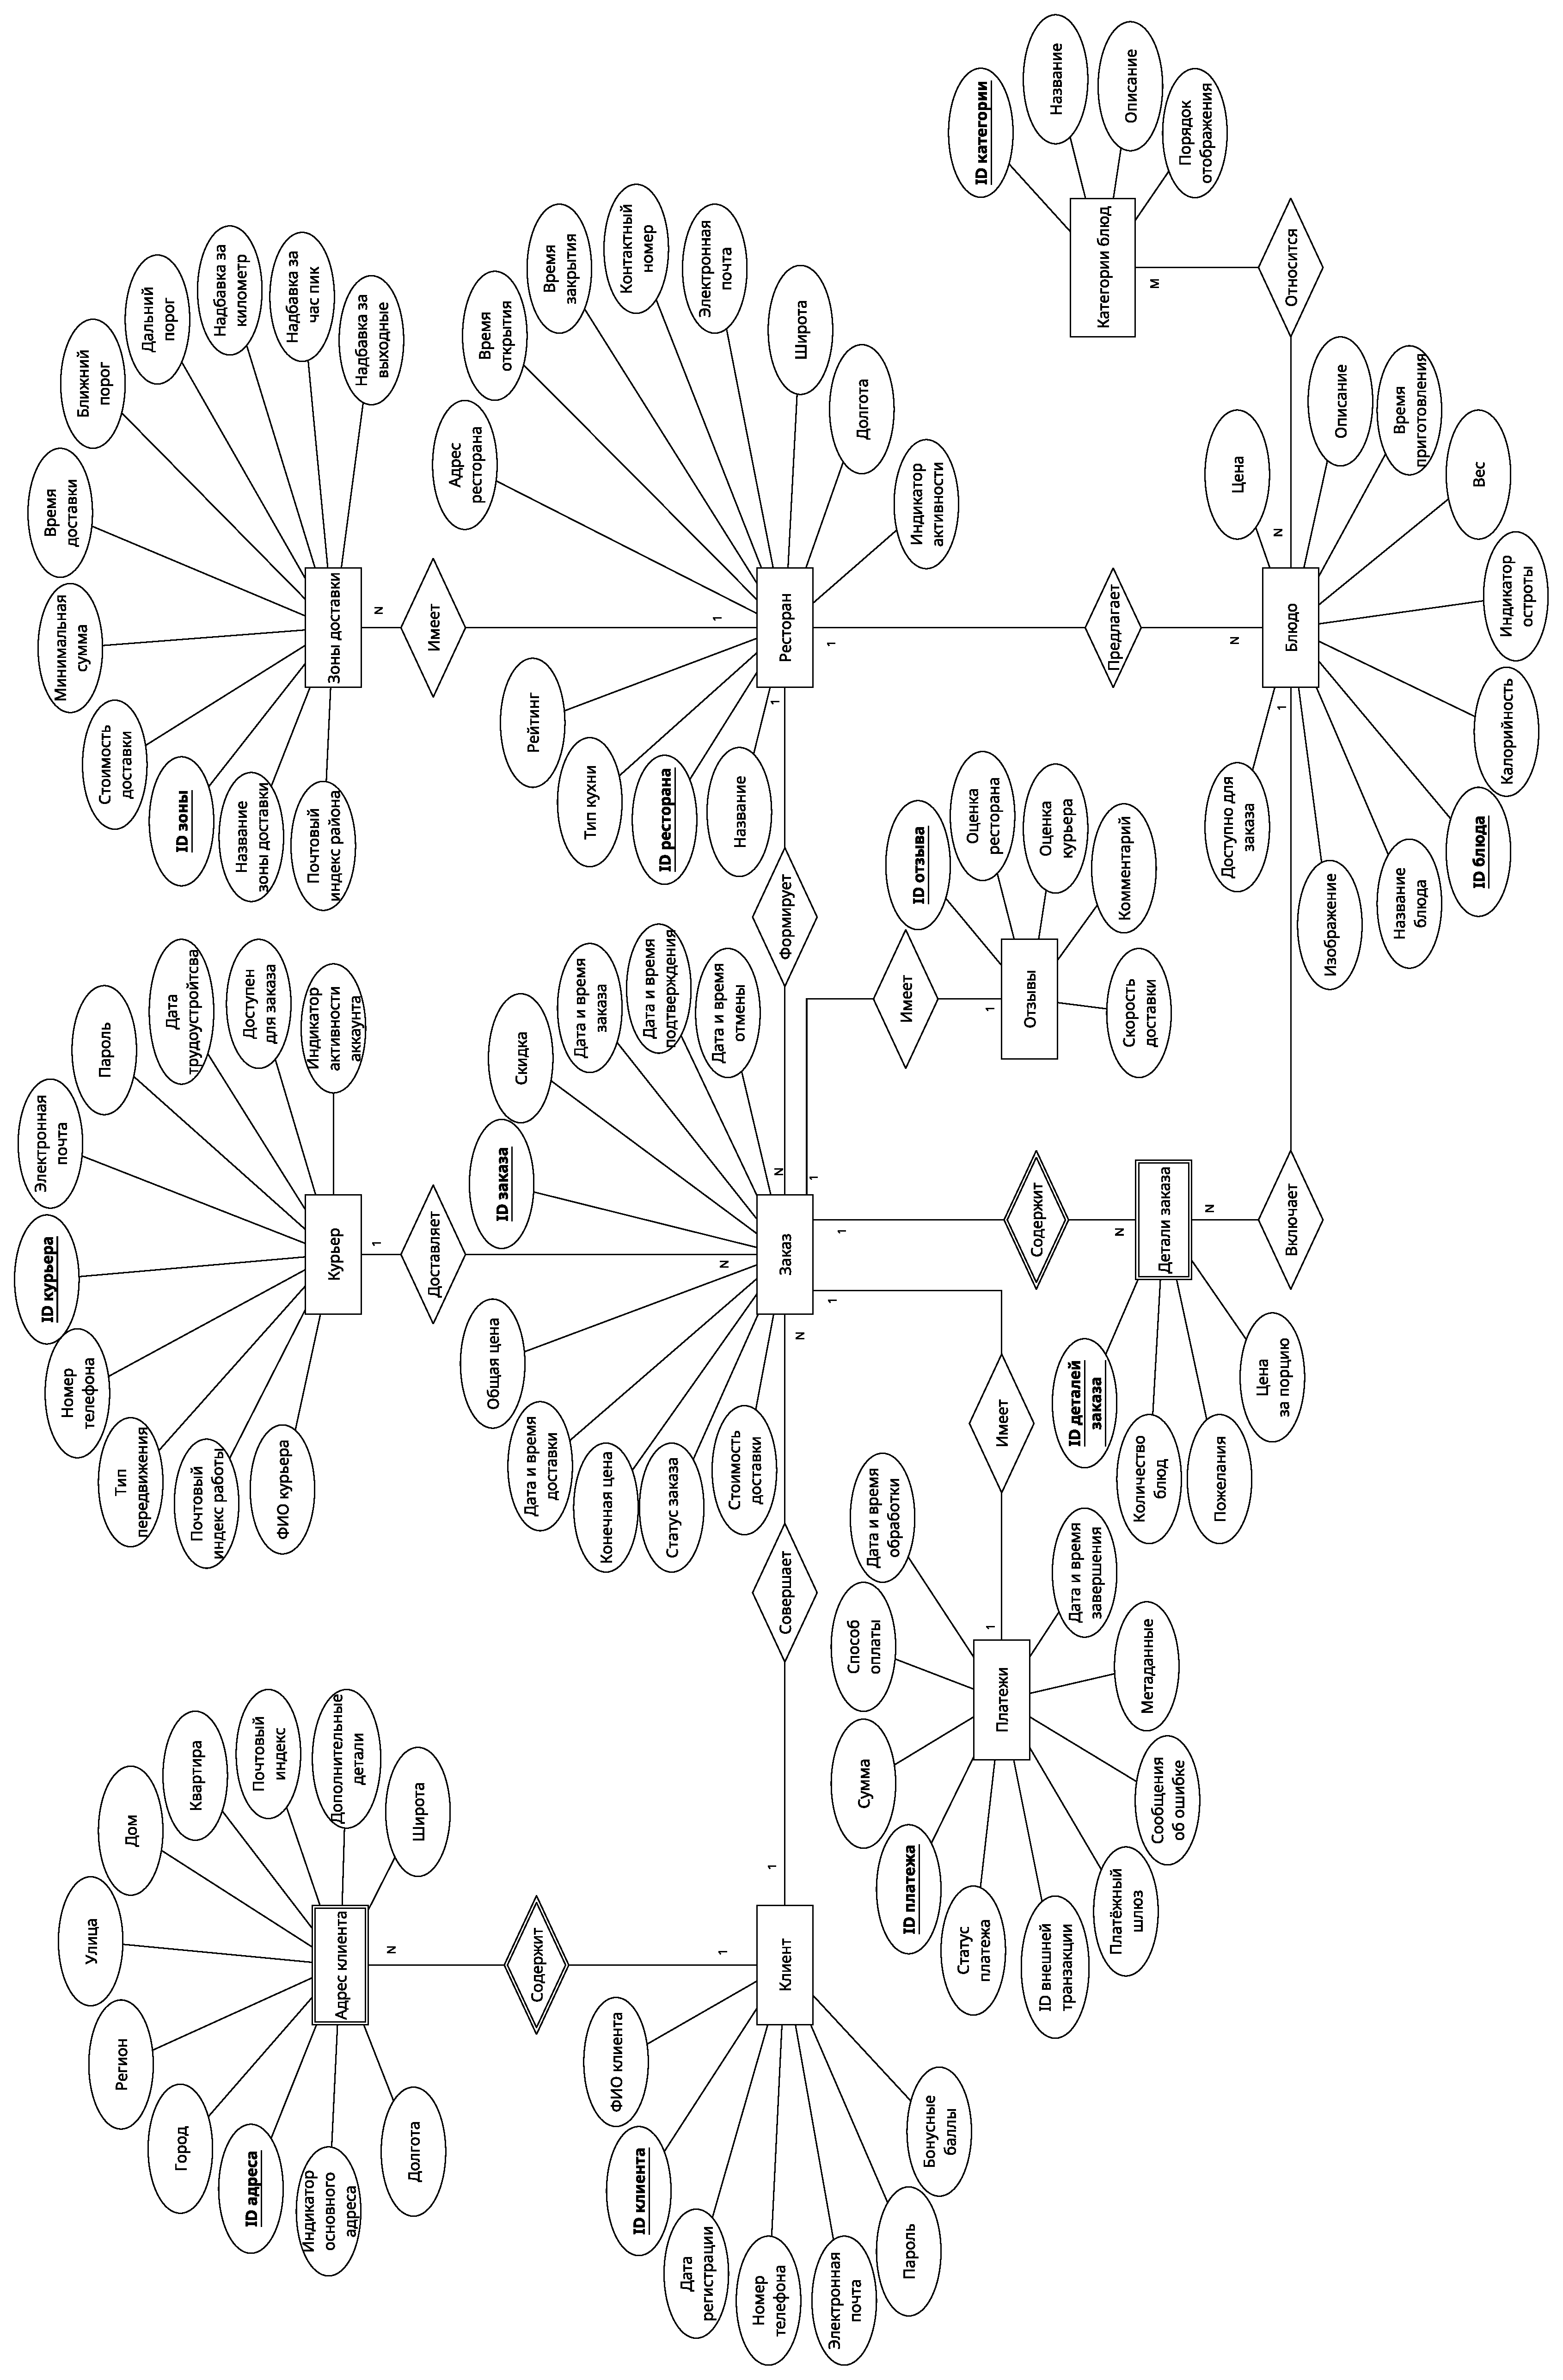
\includegraphics[width=\textwidth]{img/er-diagram_rotate.pdf}
    \caption{Диаграмма сущность-связь}
    \label{img:er-diagram}
\end{figure}

\subsection{Анализ моделей данных}
Дореляционные модели представлены инвертированными списками, иерархической и сетевой моделями. Иерархическая модель организует данные в виде дерева, где каждый дочерний узел имеет ровно одного родителя. Сетевая модель расширяет иерархическую, допуская наличие нескольких родительских узлов. Инвертированные списки представляют данные в виде таблиц, но для поисковых атрибутов создаются отдельные индексы, которые содержат упорядоченные списки значений с указателями на соответствующие записи основной таблицы (инвертированный список). Это обеспечивает быстрый поиск по нескольким условиям одновременно. Иерархическая и сетевая модели обеспечивают высокую производительность
при заранее известных маршрутах доступа к данным, тогда как инвертированные списки ускоряют поиск по любому индексированному атрибуту. Однако все три модели обладают жёсткой структурой и требуют значительных затрат при модификации схемы~\cite{ref:models_db}.

Реляционная модель, предложенная Э. Коддом в 1970 году, основывается на математической теории отношений и представляет данные исключительно в виде таблиц~\cite{ref:models_db}. Связи в этой модели устанавливаются через явное задание значений атрибутов, таких как внешние ключи. Модель обеспечивает независимость данных от способов их физического хранения, поддерживает декларативный язык запросов SQL и гарантирует выполнение требований ACID через механизм транзакций. Реляционные СУБД получили доминирующее распространение благодаря своей гибкости и строгому математическому аппарату~\cite{ref:date_db}.

Постреляционные модели включают документные, графовые, столбцовые хранилища и системы типа <<ключ-значение>>. Они разрабатывались для преодоления ограничений реляционного подхода при работе со слабоструктурированными данными, необходимости горизонтального масштабирования и экстремальных нагрузках в распределенных средах. Большинство таких решений (класса NoSQL) обеспечивают высокую производительность и доступность за счет ослабления требований к транзакционности и строгой согласованности данных~\cite{ref:dbtech}.

Для разрабатываемой базы данных выбрана реляционная модель, поскольку
предметная область характеризуется чётко определёнными связями между
сущностями, необходимостью обеспечения целостности данных и поддержкой
сложных запросов с агрегацией.

\subsection{Формализация и описание пользователей}
Взаимодействовать с разрабатываемой системой онлайн-заказов еды будут следующие роли пользователей:
\begin{itemize}
    \item гость;
    \item клиент;
    \item курьер;
    \item администратор ресторана;
    \item администратор системы.
\end{itemize}

Гость~--- неавторизованный пользователь, может только просматривать рестораны и меню, но не может совершать заказы.

Клиент~--- основная роль системы, может выбрать адрес доставки, просматривать доступные рестораны и их меню, совершать заказы, просматривать историю заказов, отслеживать их статус и оставлять отзыв о заказе.

Курьер принимает назначенные заказы и управляет статусом их доставки.

Администратор ресторана управляет меню и заказами своего ресторана.

Администратор системы управляет всей платформой.

На рисунке~\ref{img:use-case} представлена диаграмма вариантов использования разрабатываемой системы.
\jimg{use-case}{Диаграмма вариантов использования}

\subsection{Вывод}
В аналитическом разделе был проведён анализ предметной области, сформулированы требования и ограничения к разрабатываемой базе данных и приложению, выделены сущности предметной области и описаны связи между ними, был проведён анализ моделей данных и была выбрана реляционная модель на основе формализации данных, выделены роли и описание пользователей системы.